\documentclass[]{standalone}

\usepackage{adjustbox}

\usepackage{amsmath}
\usepackage{xfrac}
\usepackage{mathrsfs}

\usepackage{circuitikz}
\usepackage{tikz}
\usetikzlibrary{arrows, patterns, decorations.pathmorphing, backgrounds, positioning, fit, petri, shapes, trees, matrix, chains, decorations, decorations.pathreplacing, decorations.fractals, calc,snakes,trees, decorations.markings}

\usepackage{color}
\definecolor{soton}{RGB}{7,51,71}
\colorlet{comms}{red!50!yellow}
\colorlet{payld}{pink!50!purple}
\colorlet{obdh}{green!50!black}

\begin{document}

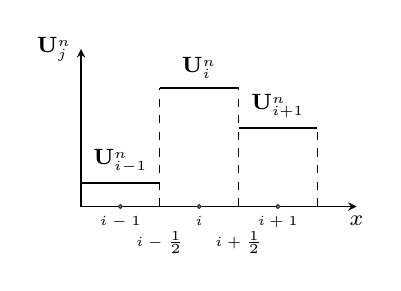
\begin{tikzpicture}

\draw[stealth-stealth] (0, 2) node[left] {\footnotesize{$\mathbf{U}$}\tiny{$_j^n$}} -- (0,0) -- (3.5,0) node[below] {\footnotesize{$x$}};

\draw[thick] (0,0.3) -- (1, 0.3);
\draw[thick] (1,1.5) -- (2,1.5);
\draw[thick] (2,1) -- (3,1);
\draw[dashed] (1,0) -- (1,1.5);
\draw[dashed] (2,0) -- (2,1.5);
\draw[dashed] (3,0) -- (3,1);

\draw[black!80, fill=black!50] (0.5, 0) node[below, black] {\tiny{$i-1$}} circle (0.025);
\draw[black!80, fill=black!50] (1.5, 0) node[below, black] {\tiny{$i$}} circle (0.025);
\draw[black!80, fill=black!50] (2.5, 0) node[below, black] {\tiny{$i+1$}} circle (0.025);

\node[below] (im) at (1,-0.2) {\tiny{$i-\tfrac{1}{2}$}};
\node[below] (ip) at (2,-0.2) {\tiny{$i+\tfrac{1}{2}$}};

\node[above] at (0.5, 0.3) {\footnotesize{$\mathbf{U}$}\tiny{$_{i-1}^n$}};
\node[above] at (1.5, 1.5) {\footnotesize{$\mathbf{U}$}\tiny{$_{i}^n$}};
\node[above] at (2.5, 1) {\footnotesize{$\mathbf{U}$}\tiny{$_{i+1}^n$}};

\end{tikzpicture}


\end{document}